\documentclass{scrreprt}

\usepackage[german]{babel}
\usepackage{libertine}
\usepackage{graphicx}
\usepackage[table,xcdraw]{xcolor} %color in tables
\usepackage{tabu}
\usepackage{hyperref}
\usepackage{array, tabularx, caption, boldline}
\usepackage{longtable}
\usepackage{ragged2e}
\usepackage{hhline}
\newcolumntype{x}[1]
{>{\raggedright}p{#1}}
\newcolumntype{z}[1]
{>{\centering}p{#1}}
\newcommand{\tn}{\tabularnewline}
\renewcommand\tabularxcolumn[1]{>{\Centering}m{#1}}  %% COMMENT
\usepackage{cellspace}
\usepackage{pdfpages} 
\setlength\cellspacetoplimit{4pt}
\setlength\cellspacebottomlimit{4pt}
\usepackage{tikz}
\newcommand*\circled[1]{\tikz[baseline=(char.base)]{
		\node[shape=circle,draw,inner sep=2pt] (char) {#1};}}

\RedeclareSectionCommand[
  beforeskip=-.5\baselineskip,
  afterskip=.25\baselineskip]{subsubsection}
\RedeclareSectionCommand[
  beforeskip=-.5\baselineskip,
  afterskip=-0.5em]{paragraph}
\RedeclareSectionCommand[
  beforeskip=-.2\baselineskip,
  afterskip=-0.5em]{subparagraph}

\title{Splatoon 2 Callouts \&  Strats}
\subtitle{Für meine liebe Lordschaft}
\author{(c) 2019 Benedikt Holler}
\date{Stand: \today \\ ver. 0.1}

\begin{document}
\maketitle
\begin{center}
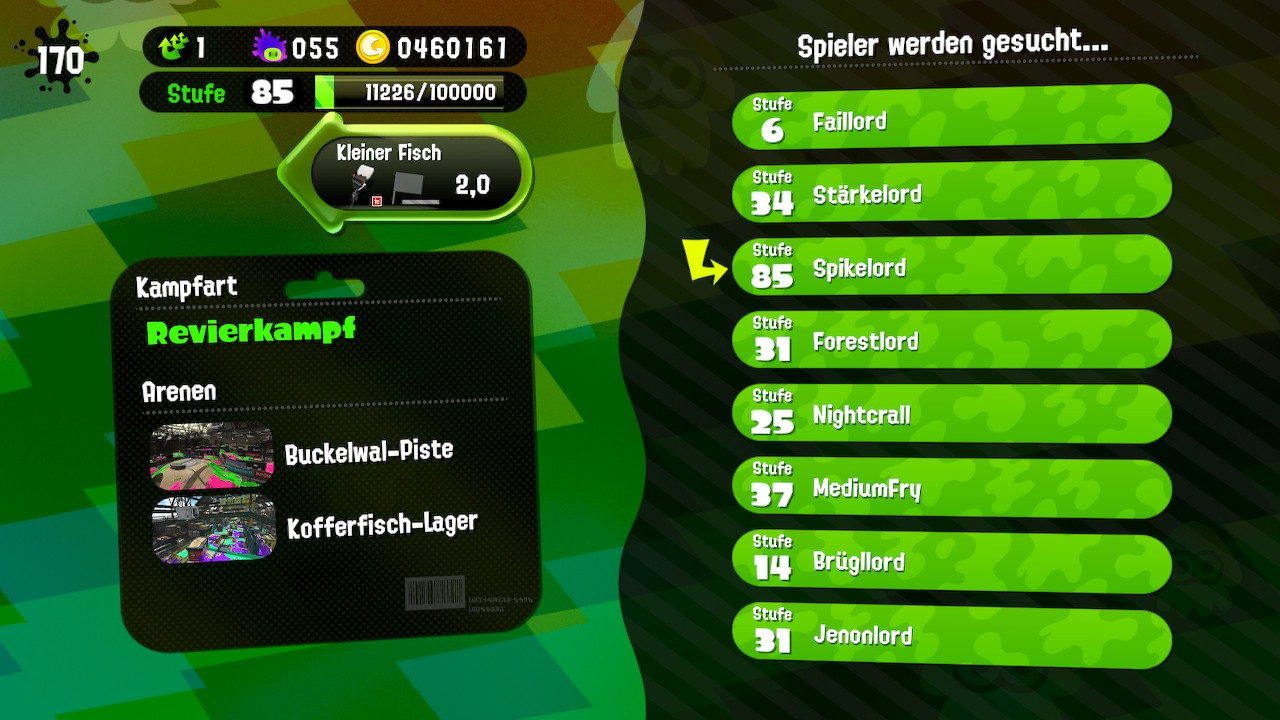
\includegraphics[width=\linewidth]{img/lerds.jpg}
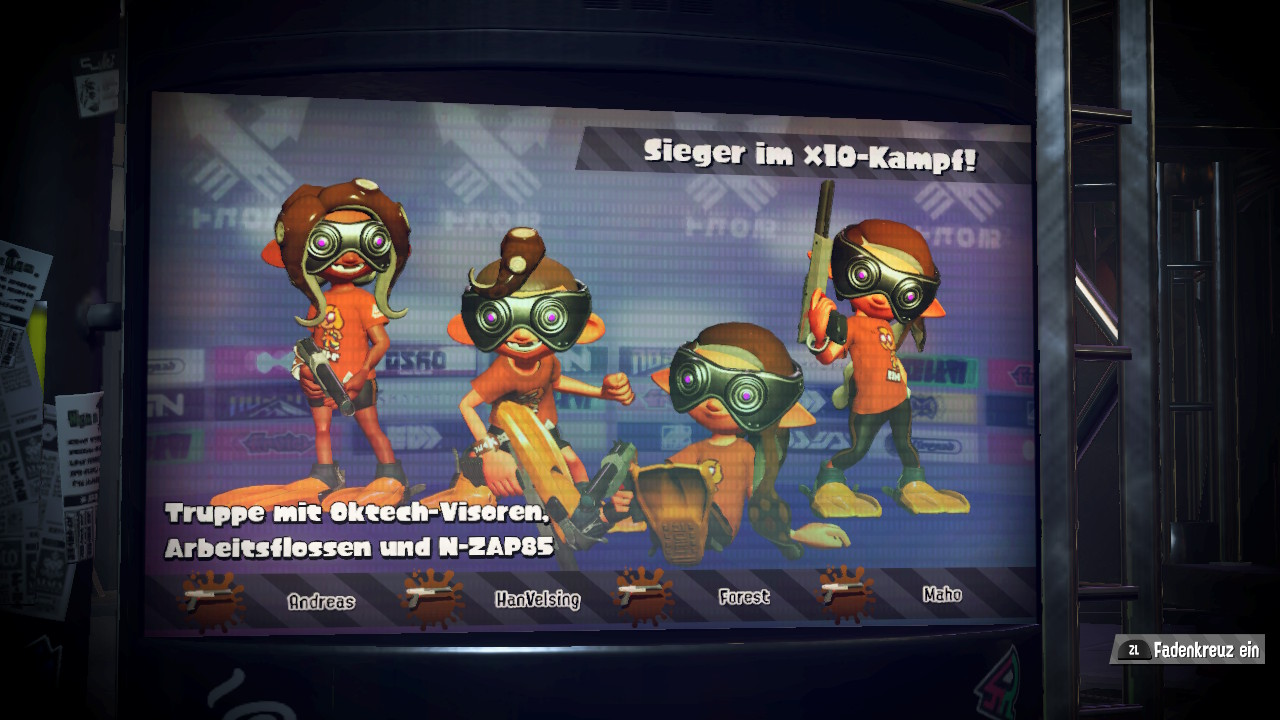
\includegraphics[width=\linewidth]{img/splatfest.jpg}
\end{center}
\tableofcontents

\chapter{Basics}
\paragraph{Positionen.} Wenn du einen Gegner siehst, am besten \emph{sofort} Bescheid geben wo er sich befindet, und welche Waffe er hat. Dann können Kollegen ihn evtl. überraschen oder dir beim Zweikampf helfen. \\
Am besten das Format benutzen: \\
Ort - Anzahl - Waffe(n) - Zusatzinfos\\
Beispiele: 
\begin{itemize}
	\item Top Mid, zwei Gegner, N-Zap und Kleckser
	\item Linker Garten, Pinsler, ist am Campen
	\item Unser Hof, Blaster, hat Inkjet bereit
	\item Ihr Close, Pro, schmeißt gleich Booyah Bomb
\end{itemize}
\paragraph{Nach dem Tod.} Wenn du stirbst, calle kurz was dich wo gekillt hat und ob du getradet hast. Mach dann am besten sofort die Karte auf und hab einen Überblick über das Geschehen. So kannst du (an den Farbklecksern die auf der Karte entstehen) erkennen, wenn sich jemand deinen Kollegen nähert. 
Beispiele: 
\begin{itemize}
	\item N-Zap hat mich, ist Links Lower Mid
	\item Eimer hat mich, ist Gay Spot, geht jetzt Hof
	\item Hab mit Blobbi getradet
	\item Magda, zu dir kommt Pro
	\item Jemand sneakt zu unserem Spawn, vermutlich Kleckser
	\item Splatling hat mich, hat jetzt Special
\end{itemize}
\paragraph{Kooperation.} Splatoon ist ein Team-Spiel :). Neben den allgemeinen Strats die hier evtl. mal aufgelistet sind kann es hilfreich sein, zu zweit an ein gewisses Ziel heranzugehen. Am besten ist es hier, wen der Support-Spieler mit einem Slayer zusammen geht, da der Backliner seine Position halten sollte und meistens nicht so gut pushen kann.
\begin{itemize}
	\item Andreas, wir beide pushen Main
	\item Bene, wir pressuren Top Mid, du gehts links, ich rechts
	\end{itemize}
\paragraph{Special-Synergien.} Immer bedenken: \textbf{Specials gewinnen Spiele!} Wenn zwei, oder sogar drei Specials zeitgleich sinnvoll genutzt werden kann der Gegner gehörig unter Druck gesetzt werden und ein Push vollkommen eliminiert werden. \\
Was daher wichtig ist: Wenn du als letzter lebst, \textbf{Versuch, am Leben zu bleiben!} Dein Team hat gerade einen Großteil ihrer Specials durch den Tod verloren, während die Gegner langsam aber sicher ihre aufbauen. Wenn du überlebst und durch deinen Special einen Push aufhalten kannst, bedeutet das einen großem Momentum Swing. \\
Ebenso sind Specials hervorragend geeignet, um das Spiel zu seinen Gunsten zu entscheiden. Bei zwei oder drei aktiven Specials ist der Gegner oftmals schlicht machtlos. Einige gute Synergien sind: 
\begin{itemize}
	\item Mehrere Jetpacks
	\item Tintenrüstung und offensive Specials
	\item Blasen und Regen
	\item Laser und absolut alles im Spiel! (srsly, der Laser ist einer der Hauptgründe, einen Backliner zu haben)
\end{itemize}
Damit die Special-Kooperation funktioniert, ist natürlich wie bei allem die Kommunikation wichtig. Gib regelmäßig Bescheid wie weit dein Special ist und sprich dich mit deinem Team ab, damit ihr das meiste aus ihnen herausholt.
\chapter{Waffen-Callouts}
\section{Hauptwaffen}
\begin{center}
\begin{longtable}{|m{3.5cm}|m{4cm}|m{4cm}|m{2cm}|}
\hline
\textbf{Waffe} & \textbf{Name (Englisch)} & \textbf{Name (Deutsch)} & \textbf{Vorschlag Abkürzung} \\ \hline
\hline
\endfirsthead
\hline
\textbf{Waffe} & \textbf{Name (Englisch)} & \textbf{Name (Deutsch)} & \textbf{Vorschlag Abkürzung} \\ \hline
\hline
\endhead
    \parbox[c]{10em}{ 
    	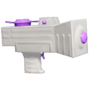
\includegraphics[height=1cm]{img/splattershotjunior.png} 
		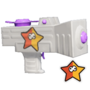
\includegraphics[height=1cm]{img/customsplattershotjunior.png} 
		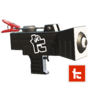
\includegraphics[height=1cm]{img/kensasplattershotjunior.png}
	} &  
    Splattershot Jr., Custom Splattershot Jr., Kensa Splattershot Jr.  &
	Junior-Kleckser, Junior-Kleckser Plus, Kensa-Junior-Kleckser&
	Junior 
	\\ \hline
	\parbox[c]{10em}{
		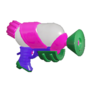
\includegraphics[height=1cm]{img/splattershot.png} 
		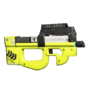
\includegraphics[height=1cm]{img/heroshotreplica.png} 
		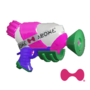
\includegraphics[height=1cm]{img/tentateksplattershot.png}} \parbox[c]{10em}{
		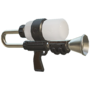
\includegraphics[height=1cm]{img/octoshotreplica.png} 
		
\includegraphics[height=1cm]{img/kensasplattershot.png} 
	} &
Splattershot, Hero Shot Replica, Tentatek Splattershot, Octo Shot Replica, Kensa Splattershot  
Kleckser &
	Kleckser, Heldenwaffe Replik, Tentatek-Kleckser, Okto-Kleckser Replik, Kensa-Kleckser &
	Kleckser
	\\ \hline
	\parbox[c]{10em}{
		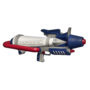
\includegraphics[height=1cm]{img/splattershotpro.png} 
		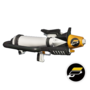
\includegraphics[height=1cm]{img/forgesplattershotpro.png} 
		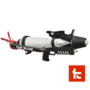
\includegraphics[height=1cm]{img/kensasplattershotpro.png}}
	& Splattershot Pro, Forge Splattershot Pro, Kensa Splattershot Pro
	& Profi-Kleckser, Focus-Profi-Kleckser, Kensa-Profi-Kleckser
	& Pro
	\\ \hline
	\parbox[c]{10em}{
		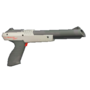
\includegraphics[height=1cm]{img/nzap85.png} 
		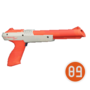
\includegraphics[height=1cm]{img/nzap89.png}
	}
	& N-Zap '85, N-Zap '89
	& N-Zap '85, N-Zap '89
	& N-Zap
	\\ \hline
	\parbox[c]{10em}{
		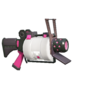
\includegraphics[height=1cm]{img/52gal.png} 
		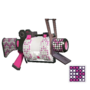
\includegraphics[height=1cm]{img/52galdeco.png} 
		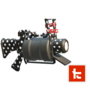
\includegraphics[height=1cm]{img/kensa52gal.png}}
	& .52 Gal, .52 Gal Deco, Kensa .52 Gal
	& .52 Gallon, .52 Gallon Deko, Kensa .52 Gallon
	& Gal
	\\ \hline
	\parbox[c]{10em}{
		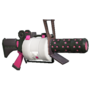
\includegraphics[height=1cm]{img/96gal.png} 
		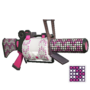
\includegraphics[height=1cm]{img/96galdeco.png}
	}
	& .96 Gal, .96 Gal Deco
	& .96 Gallon, .96 Gallon Deko
	& Big Gal
	\\ \hline
	\parbox[c]{10em}{
		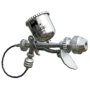
\includegraphics[height=1cm]{img/aerospraymg.png} 
		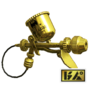
\includegraphics[height=1cm]{img/aerosprayrg.png}
	}
	& Aerospray MG, Aerospray RG
	& Aerospray MG, Aerospray RG
	& Aero(spray)
	\\ \hline
	\parbox[c]{10em}{
		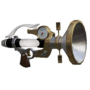
\includegraphics[height=1cm]{img/splooshomatic.png} 
		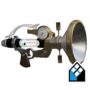
\includegraphics[height=1cm]{img/neosplooshomatic.png}
	}
	& Sploosh-o-matic, Neo Sploosh-o-matic
	& Disperser, Disperser Neo
	& Sploosh
	\\ \hline
	\parbox[c]{10em}{
		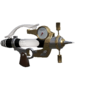
\includegraphics[height=1cm]{img/splashomatic.png} 
		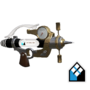
\includegraphics[height=1cm]{img/neosplashomatic.png}
	}
	& Splash-o-matic, Neo Splash-o-matic
	& Fein-Disperser, Fein-Disperser Neo
	& Splash
	\\ \hline
	\parbox[c]{10em}{
		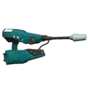
\includegraphics[height=1cm]{img/jetsquelcher.png} 
		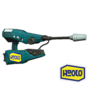
\includegraphics[height=1cm]{img/customjetsquelcher.png}
	}
	& Jet Squelcher, Custom Jet Squelcher
	& Platscher, Platscher SE
	& Jet
	\\ \hline
	\parbox[c]{10em}{
		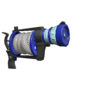
\includegraphics[height=1cm]{img/l3nozzlenose.png} 
		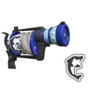
\includegraphics[height=1cm]{img/l3nozzlenosed.png} 
		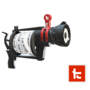
\includegraphics[height=1cm]{img/kensal3nozzlenose.png}}
	& L-3 Nozzlenose, L-3 Nozzlenose D, Kensa L-3 Nozzlenose
	& L3 Tintenwerfer, L3 Tintenwerfer D, Kensa-L3 Tintenwerfer
	& L3
	\\ \hline	
	\parbox[c]{10em}{
		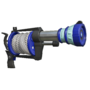
\includegraphics[height=1cm]{img/h3nozzlenose.png} 
		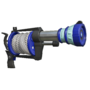
\includegraphics[height=1cm]{img/h3nozzlenose.png}
	}
	& H-3 Nozzlenose, H-3 Nozzlenose D
	& H3-Tintenwerfer, H3-Tintenwerfer D
	& H3
	\\ \hline
	\parbox[c]{10em}{
		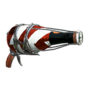
\includegraphics[height=1cm]{img/squeezer.png} 
		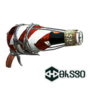
\includegraphics[height=1cm]{img/foilsqueezer.png}
	}
	& Squeezer, Foil Squeezer
	& Quetscher, Quetscher Fol
	& Squeezer
	\\ \hline
	\parbox[c]{10em}{
		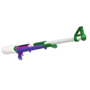
\includegraphics[height=1cm]{img/splatcharger.png} 
		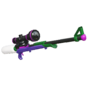
\includegraphics[height=1cm]{img/splatterscope.png} 
		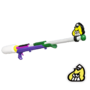
\includegraphics[height=1cm]{img/firefinsplatcharger.png}} \parbox[c]{10em}{
		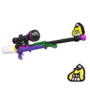
\includegraphics[height=1cm]{img/firefinsplatterscope.png} 
		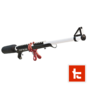
\includegraphics[height=1cm]{img/kensacharger.png} 
		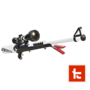
\includegraphics[height=1cm]{img/kensasplatterscope.png} 
	} 
	& Splat Charger, Splatterscope,  Firefin Splat Charger, Firefin Splatterscope, Kensa Charger, Kensa Splatterscope 
	& Konzentrator, Ziel-Konzentrator, Rilax-Konzentrator, Rilax-Ziel-Konzentrator, Kensa-Konzentrator, Kensa-Ziel-Konzentrator
	& Charger
	\\ \hline	
	\parbox[c]{10em}{
		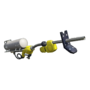
\includegraphics[height=1cm]{img/eliter4k.png} 
		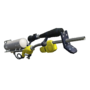
\includegraphics[height=1cm]{img/eliter4kscope.png} 
		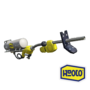
\includegraphics[height=1cm]{img/customeliter4k.png}} \parbox[c]{10em}{
		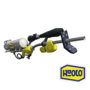
\includegraphics[height=1cm]{img/customeliter4kscope.png}
	} 
	& E-Liter 4k, E-Liter 4k Scope, Custom E-Liter 4k, Custom E-Liter 4k Scope
	& E-Liter 4k, Ziel-E-Liter 4k, E-Liter 4k SE, Ziel-E-Liter 4k SE
	& (E-)Liter
	\\ \hline
	\parbox[c]{10em}{
		
\includegraphics[height=1cm]{img/classicsquiffer.png} 
		
\includegraphics[height=1cm]{img/newsquiffer.png}
	}
	& Classic Squiffer, New Squiffer
	& Sepiator a, Sepiator b
	& Squiffer
	\\ \hline	
	\parbox[c]{10em}{
		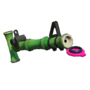
\includegraphics[height=1cm]{img/bamboozler14mk1.png} 
		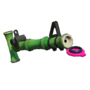
\includegraphics[height=1cm]{img/bamboozler14mk2.png}
	}
	& Bamboozler 14 MK I, Bamboozler 14 MK 2
	& Klotzer 14-A, Klotzer 14-B
	& Bamboozler
	\\ \hline
	\parbox[c]{10em}{
		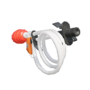
\includegraphics[height=1cm]{img/gootuber.png} 
		\includegraphics[height=1cm]{img/customgootuber.png}
	}
	& Goo Tuber, Custom Goo Tuber
	& T-Tuber, T-Tuber SE
	& Goo-Tube
	\\ \hline
	\parbox[c]{10em}{
		\includegraphics[height=1cm]{img/splatroller.png} 
		\includegraphics[height=1cm]{img/herorollerreplica.png} 
		\includegraphics[height=1cm]{img/krakonsplatroller.png}} \parbox[c]{10em}{
		\includegraphics[height=1cm]{img/kensasplatroller.png}
	} 
	& Splat Roller, Hero Roller Replica, Krak-On Splat Roller, Kensa Splat Roller
	& Klecksroller, Helden-Roller Replik, Medusa-Klecksroller, Kensa-Klecksroller
	& Roller
	\\ \hline
	\parbox[c]{10em}{
		\includegraphics[height=1cm]{img/carbonroller.png} 
		\includegraphics[height=1cm]{img/carbonrollerdeco.png}
	}
	& Carbon Roller, Carbon Roller Deco
	& Karbnroller, Karbonroller Deko
	& Karbon
	\\ \hline
	\parbox[c]{10em}{	
		\includegraphics[height=1cm]{img/dynamoroller.png} 
		\includegraphics[height=1cm]{img/golddynamoroller.png} 
		\includegraphics[height=1cm]{img/kensadynamoroller.png}}
	& Dynamo Roller, Gold Dynamo Roller, Kensa Dynamo Roller
	& Dynaroller, Dynaroller Tesla, Kensa-Dynaroller
	& Döner
	\\ \hline
	\parbox[c]{10em}{
		\includegraphics[height=1cm]{img/flingzaroller.png} 
		\includegraphics[height=1cm]{img/foilflingzaroller.png}
	}
	& Flingza Roller, Foil Flingza Roller
	& Flex-Roller, Flex-Roller Fol
	& Flex, Flingza
	\\ \hline	
	\parbox[c]{10em}{
	\includegraphics[height=1cm]{img/splatdualies.png} 
	\includegraphics[height=1cm]{img/herodualiereplicas.png} 
	\includegraphics[height=1cm]{img/enperrysplatdualies.png}} \parbox[c]{10em}{
	\includegraphics[height=1cm]{img/kensasplatdualies.png}
} 
& Splat Dualies, Hero Dualie Replicas, Enperry Splat Dualies, Kensa Splat Dualies
& Klecks-Doppler, Helden-Doppler Replik, Enperry-Klecks-Doppler, Kensa-Klecks-Doppler
& Dualies
\\ \hline
\parbox[c]{10em}{
	\includegraphics[height=1cm]{img/dualiesquelcher.png} 
	\includegraphics[height=1cm]{img/customdualiesquelcher.png}
}
& Dualie Squelchers, Custom Dualie Squelchers
& Doppel-Platscher, Doppel-Platscher SE
& Squelchies
\\ \hline
\parbox[c]{10em}{
	\includegraphics[height=1cm]{img/dappledualies.png} 
	\includegraphics[height=1cm]{img/dappledualiesnouveau.png}
}
& Dapple Dualies, Dapple Dualies Nouveau
& Sprenkler, Sprenkler Fresco
& Dapples
\\ \hline
\parbox[c]{10em}{
	\includegraphics[height=1cm]{img/gloogadualies.png} 
	\includegraphics[height=1cm]{img/gloogadualiesdeco.png} 
	\includegraphics[height=1cm]{img/kensagloogadualies.png}}
& Glooga Dualies, Glooga Dualies Deco, Kensa Glooga Dualies
& Kelvin 525, Kelvin 525 Deko, Kensa-Kelvin 525
& Gloogas
\\ \hline
\parbox[c]{10em}{
	\includegraphics[height=1cm]{img/darktetradualies.png} 
	\includegraphics[height=1cm]{img/lighttetradualies.png}
}
& Dark Tetra Dualies, Light Tetra Dualies
& Quadhopper Noir, Quadhopper Blanc
& Tetra
\\ \hline	
	\parbox[c]{10em}{
		\includegraphics[height=1cm]{img/blaster.png} 
		\includegraphics[height=1cm]{img/heroblasterreplica.png} 
		\includegraphics[height=1cm]{img/customblaster.png}}
	& Blaster, Hero Blaster Replica, Custom Blaster
	& Blaster, Helden-Blaster Replik, Blaster SE
	& Blaster
	\\ \hline
	\parbox[c]{10em}{
		\includegraphics[height=1cm]{img/rangeblaster.png} 
		\includegraphics[height=1cm]{img/customrangeblaster.png}
	}
	& Range Blaster, Custom Range Blaster
	& Fern-Blaster, Fern-Blaster SE
	& Range
	\\ \hline
	\parbox[c]{10em}{	
		\includegraphics[height=1cm]{img/lunablaster.png} 
		\includegraphics[height=1cm]{img/lunablasterneo.png} 
		\includegraphics[height=1cm]{img/kensalunablaster.png}}
	& Luna Blaster, Luna Blaster Neo, Kensa Luna Blaster
	& Luna-Blaster, Luna-Blaster Neo, Kensa-Luna-Blaster
	& Luna
	\\ \hline	
	\parbox[c]{10em}{
		\includegraphics[height=1cm]{img/rapidblaster.png} 
		\includegraphics[height=1cm]{img/rapidblasterdeco.png} 
		\includegraphics[height=1cm]{img/kensarapidblaster.png}}
	& Rapid Blaster, Rapid Blaster Deco, Kensa Rapid Blaster
	& Turbo-Blaster, Turbo-Blaster Deko, Kensa-Turbo-Blaster
	& Rapid
	\\ \hline
	\parbox[c]{10em}{
		\includegraphics[height=1cm]{img/rapidblasterpro.png} 
		\includegraphics[height=1cm]{img/rapidblasterprodeco.png}
	}
	& Rapid Blaster Pro, Rapid Blaster Pro Deco
	& Turbo-Blaster Pro, Turbo-Blaster Pro Deco
	& Rapid Pro
	\\ \hline
	\parbox[c]{10em}{
		\includegraphics[height=1cm]{img/clashblaster.png} 
		\includegraphics[height=1cm]{img/clashblasterneo.png}
	}
	& Clash Blaster, Clash Blaster Neo
	& Kontra-Blaster, Kontra-Blaster Neo
	& Kontra
	\\ \hline
	\parbox[c]{10em}{
		\includegraphics[height=1cm]{img/slosher.png} 
		\includegraphics[height=1cm]{img/heroslosherreplica.png} 
		\includegraphics[height=1cm]{img/slosherdeco.png}}
	& Slosher, Hero Slosher Replica, Slosher Deco
	& Schwapper, Helden-Schwapper Replik, Schwapper Deko
	& Eimer
	\\ \hline
	\parbox[c]{10em}{
		\includegraphics[height=1cm]{img/trislosher.png} 
		\includegraphics[height=1cm]{img/trisloshernouveau.png}
	}
	& Tri Slosher, Tri Slosher Nouveau
	& 3R-Schwapper, 3R-Schwapper Fresco
	& Tri
	\\ \hline
	\parbox[c]{10em}{
		\includegraphics[height=1cm]{img/sloshingmachine.png} 
		\includegraphics[height=1cm]{img/sloshingmachineneo.png} 
		\includegraphics[height=1cm]{img/kensasloshingmachine.png}}
	& Sloshing Machine, Sloshing Machine Neo, Kensa Sloshing Machine
	& Trommel-Schwapper, Trommel-Schwapper Neo, Kensa-Trommel-Schwapper
	& Sloshing
	\\ \hline
	\parbox[c]{10em}{
		\includegraphics[height=1cm]{img/explosher.png} 
		\includegraphics[height=1cm]{img/customexplosher.png}
	}
	& Explosher, Custom Explosher
	& Knall-Schwapper, Knapp-Schwapper SE
	& Heizung
	\\ \hline
	\parbox[c]{10em}{
		\includegraphics[height=1cm]{img/bloblobber.png} 
		\includegraphics[height=1cm]{img/bloblobberdeco.png}
	}
	& Bloblobber, Bloblobber Deco
	& Wannen-Schwapper, Wannen-Schwapper Deko
	& Blobbi
	\\ \hline
	\parbox[c]{10em}{
		\includegraphics[height=1cm]{img/inkbrush.png} 
		\includegraphics[height=1cm]{img/inkbrushnouveau.png}}
	& Inkbrush, Inkbrush Nouveau
	& Quasto, Quasto Fresco
	& Pinsler
	\\ \hline
	\parbox[c]{10em}{
		\includegraphics[height=1cm]{img/octobrush.png} 
		\includegraphics[height=1cm]{img/herobrushreplica.png} 
		\includegraphics[height=1cm]{img/octobrushnouveau.png}} \parbox[c]{10em}{
		\includegraphics[height=1cm]{img/kensaoctobrush.png}
	} 
	& Octobrush, Herobrush Replica, Octobrush Nouveau, Kensa Octobrush
	& Kalligraf, Helden-Pinsel Replik, Kalligraf Fresco, Kensa-Kalligraf
	& Octo
	\\ \hline
	\parbox[c]{10em}{
		\includegraphics[height=1cm]{img/heavysplatling.png} 
		\includegraphics[height=1cm]{img/herosplatlingreplica.png} 
		\includegraphics[height=1cm]{img/heavysplatlingdeco.png}}
	& Heavy Splatling, Hero Splatling Replica, Heavy Splatling Deco
	& Splatling, Helden-Splatling Replik, Splatling Deko
	& Splatling
	\\ \hline
	\parbox[c]{10em}{
		\includegraphics[height=1cm]{img/minisplatling.png} 
		\includegraphics[height=1cm]{img/zinkminisplatling.png} 
		\includegraphics[height=1cm]{img/kensaminisplatling.png}}
	& Mini Splatling, Zink Mini Splatling, Kensa Mini Splatling
	& Klecks-Spatling, Sagitron-Klecks-Splatling, Kensa-Klecks-Splatling
	& Mini
	\\ \hline
	\parbox[c]{10em}{
		\includegraphics[height=1cm]{img/hydrasplatling.png} 
		\includegraphics[height=1cm]{img/customhydrasplatling.png}
	}
	& Hydra Splatling, Custom Hydra Splatling
	& Hydrant, Hydrant SE
	& Hydra
	\\ \hline
	\parbox[c]{10em}{
		\includegraphics[height=1cm]{img/ballpointsplatling.png} 
		\includegraphics[height=1cm]{img/ballpointsplatlingnouveau.png}
	}
	& Ballpoint Splatling, Ballpoint Splatling Nouveau
	& Kuli-Splatling, Kuli-Splatling Fresco
	& Kuli
	\\ \hline
	\parbox[c]{10em}{
		\includegraphics[height=1cm]{img/nautilus47.png} 
		\includegraphics[height=1cm]{img/nautilus79.png}
	}
	& Nautilus 47, Nautilus 79
	& Nautilus 47, Nautilus 79
	& Nautilus
	\\ \hline
	\parbox[c]{10em}{
		\includegraphics[height=1cm]{img/splatbrella.png} 
		\includegraphics[height=1cm]{img/herobrellareplica.png} 
		\includegraphics[height=1cm]{img/sorellabrella.png}}
	& Splat Brella, Hero Brella Replica, Sorella Brella
	& Parapluviator, Helden-Pluviator Replik, Sorella-Parapluviator
	& Schirm
	\\ \hline
	\parbox[c]{10em}{
		\includegraphics[height=1cm]{img/tentabrella.png} 
		\includegraphics[height=1cm]{img/tentasorellabrella.png}
	}
	& Tenta Brella, Tenta Sorella Brella
	& Camp-Pluviator, Sorella-Camp-Pluviator
	& Tenta
	\\ \hline
\parbox[c]{10em}{
	\includegraphics[height=1cm]{img/undercoverbrella.png} 
	\includegraphics[height=1cm]{img/undercoversorellabrella.png} 
	\includegraphics[height=1cm]{img/kensaundercoverbrella.png}}
& Undercover Brella, Undercover Sorella Brella, Kensa Undercover Brella
& UnderCover, Sorella-UnderCover, Kensa-UnderCover
& UnderCover
\\ \hline	
\end{longtable}
\end{center}
\newpage
\section{Sekundärwaffen}
\begin{center}
	\begin{longtable}{|m{3.5cm}|m{4cm}|m{4cm}|m{2cm}|}
		\hline
		\textbf{Waffe} & \textbf{Name (Englisch)} & \textbf{Name (Deutsch)} & \textbf{Vorschlag Abkürzung} \\ \hline
		\hline
		\endfirsthead
		\hline
		\textbf{Waffe} & \textbf{Name (Englisch)} & \textbf{Name (Deutsch)} & \textbf{Vorschlag Abkürzung} \\ \hline
		\hline
		\endhead
		\hline
		\includegraphics[height=1cm]{img/splatbomb.png} & Splat Bomb & Klecksbombe & Bombe \\ \hline
		\includegraphics[height=1cm]{img/suctionbomb.png} & Suction Bomb & Haftbombe & \textbf{SUCC} \\ \hline
		\includegraphics[height=1cm]{img/burstbomb.png} & Burst Bomb & Instabombe & Insta / Burst \\ \hline
		\includegraphics[height=1cm]{img/curlingbomb.png} & Curling Bomb & Curling-Bombe & Curling \\ \hline
		\includegraphics[height=1cm]{img/autobomb.png} & Autobomb & Robo-Bombe & Robo \\ \hline
		\includegraphics[height=1cm]{img/inkmine.png} & Ink Mine & Tintenmine & Mine\\ \hline
		\includegraphics[height=1cm]{img/sprinkler.png} & Sprinkler & Sprinkler & Sprinkler \\ \hline
		\includegraphics[height=1cm]{img/toxicmist.png} & Toxic Mist & Sepitox-Nebel & Nebel \\ \hline
		\includegraphics[height=1cm]{img/pointsensor.png} & Point Sensor & Detektor & Sensor \\ \hline
		\includegraphics[height=1cm]{img/splashwall.png} & Splash Wall & Tintenwall & Wall \\ \hline
		\includegraphics[height=1cm]{img/squidbeakon.png} & Squid Beakon & Sprungboje & Beakon \\ \hline
		\includegraphics[height=1cm]{img/fizzybomb.png} & Fizzy Bomb & Soda-Bombe & Soda \\ \hline
		\includegraphics[height=1cm]{img/torpedo.png} & Torpedo & Torpedo & Torpedo \\ \hline
	\end{longtable}
\end{center}
\newpage
\section{Specials}
\begin{center}
	\begin{longtable}{|m{3.5cm}|m{4cm}|m{4cm}|m{2cm}|}
		\hline
		\textbf{Waffe} & \textbf{Name (Englisch)} & \textbf{Name (Deutsch)} & \textbf{Vorschlag Abkürzung} \\ \hline
		\hline
		\endfirsthead
		\hline
		\textbf{Waffe} & \textbf{Name (Englisch)} & \textbf{Name (Deutsch)} & \textbf{Vorschlag Abkürzung} \\ \hline
		\hline
		\endhead
		\hline
		\includegraphics[height=1cm]{img/tentamissiles.png} & Tenta Missiles & Schwarmraketen & Raketen \\ \hline
		\includegraphics[height=1cm]{img/inkarmor.png} & Ink Armor & Tintenrüstung & Rüstung \\ \hline
		\includegraphics[height=1cm]{img/bomblauncher.png} & Bomb Launcher & Bomber & Bombenspam \\ \hline
		\includegraphics[height=1cm]{img/stingray.png} & Sting Ray & Hochdruckverunreiniger & Laser \\ \hline
		\includegraphics[height=1cm]{img/inkjet.png} & Inkjet & Tintendüser & Jetpack \\ \hline
		\includegraphics[height=1cm]{img/splashdown.png} & Splashdown & Tintenschock & Splashdown \\ \hline
		\includegraphics[height=1cm]{img/inkstorm.png} & Ink Storm & Tintenschauer & Regen \\ \hline
		\includegraphics[height=1cm]{img/baller.png} & Baller & Sepisphäre & Baller \\ \hline
		\includegraphics[height=1cm]{img/bubbleblower.png} & Bubble Blower & Blasenwerfer & Blasen \\ \hline
		\includegraphics[height=1cm]{img/booyahbomb.png} & Booyah Bomb & Cool-Kugel & Booyah Bomb \\ \hline
		\includegraphics[height=1cm]{img/ultrastamp.png} & Ultra Stamp & Ultra-Stempel & Hammer \\ \hline
	\end{longtable}
\end{center}
\chapter{Maps}
\textbf{Alle Karten können auch als PNG-Files mit deutschem Namen im Ordner img/maps gefunden werden.}
\section{Korallenviertel / The Reef}
\includegraphics[width=\linewidth]{img/thereef.png}
\section{Molluskelbude / Musselforge Fitness}
\includegraphics[width=\linewidth]{img/musselforgefitness.png}
\section{Seeigel-Rockbühne / Starfish Mainstage}
\includegraphics[width=\linewidth]{img/starfishmainstage.png}
\section{Buckelwal-Piste / Humpback Pump Track}
\includegraphics[width=\linewidth]{img/humpbackpumptrack.png}
\section{Perlmutt-Akademie / Inkblot Art Academy}
\subsection{Callouts}
\includegraphics[width=\linewidth]{img/inkblotartacademy.png}
\subsection{Strats}
\paragraph{Rollout für Splat Zones, Rainmaker und Tower Control.} Slayer 1 geht über Heaven durch den linken Garten zu ihrem Main und versucht, in ihrem Hof Kills zu machen. Slayer 2 und Support pushen Mid und contesten das Objective. Backline achtet auf den rechten Garten und unser Main und callt/verhindert Flanks.
\section{Muränentürme / Moray Towers}
\includegraphics[width=\linewidth]{img/moraytowers.png}
\section{Heilbutt-Hafen / Port Mackerel}
\includegraphics[width=\linewidth]{img/portmackerel.png}
\section{Störwerft / Sturgeon Shipyard}
\includegraphics[width=\linewidth]{img/sturgeonshipyard.png}
\section{Manta Maria}
\includegraphics[width=\linewidth]{img/mantamaria.png}
\section{Tümmlerkuppel / Kelp Dome}
\includegraphics[width=\linewidth]{img/kelpdome.png}
\section{Grätenkanal / Snapper Canal}
\includegraphics[width=\linewidth]{img/snappercanal.png}
\section{Punkasius-Skatepark / Blackbelly Skatepark}
\includegraphics[width=\linewidth]{img/blackbellyskatepark.png}
\section{Cetacea-Markt / MakoMart}
\includegraphics[width=\linewidth]{img/makomart.png}
\section{Kofferfisch-lager / Walleye Warehouse}
\includegraphics[width=\linewidth]{img/walleyewarehouse.png}
\section{Abyssal-Museum / Shellendorf Institute}
\includegraphics[width=\linewidth]{img/shellendorfinstitute.png}
\section{Arowana Center / Arowana Mall}
\includegraphics[width=\linewidth]{img/arowanamall.png}
\section{Backfisch-Stadion / Goby Arena}
\includegraphics[width=\linewidth]{img/gobyarena.png}
\section{Steinköhler-Grube / Piranha Pit}
\includegraphics[width=\linewidth]{img/piranhapit.png}
\section{Steinköhler-Grube / Piranha Pit - Rainmaker}
\includegraphics[width=\linewidth]{img/piranhapit-rainmaker.png}
\section{Camp Schützenfisch / Camp Triggerfish}
\includegraphics[width=\linewidth]{img/camptriggerfish.png}
\section{Flunder-Funpark / Wahoo World}
\includegraphics[width=\linewidth]{img/wahooworld.png}
\section{Hotel Neothun / New Albacore Hotel}
\includegraphics[width=\linewidth]{img/newalbacorehotel.png}
\section{Anchobit Games HQ / Ancho-V Games}
\includegraphics[width=\linewidth]{img/anchovgames.png}
\section{Grundel-Pavillon / Skipper Pavillon}
\includegraphics[width=\linewidth]{img/skipperpavillon.png}
\end{document}
